\documentclass[problems]{esg8022pset} 
  \usepackage{amsmath}
  \usepackage{amssymb}
  \usepackage{enumerate}
  \usepackage{graphicx}
  \usepackage{hyperref}
  \usepackage{mathtools}
  \usepackage[per-mode=symbol]{siunitx} %If this line is giving you trouble, try replacing per-mode with per
  \providecommand{\uvec}[1]{{\hat{\bf{#1}}}}
  \usepackage{pgf,tikz}
  \usetikzlibrary{arrows}
  \usepackage{wasysym}
  \usepackage{subfig}
  \makeatletter
  \newcommand{\interitemtext}[1]{%
    \begin{list}{}
     {\itemindent=0mm\labelsep=0mm
     \labelwidth=0mm\leftmargin=0mm
     \addtolength{\leftmargin}{-\@totalleftmargin}}
      \item #1
    \end{list}
  }
  \makeatother
  \renewcommand{\d}{\,d}
  \providecommand{\norm}[1]{\lVert#1\rVert}

  \newcommand{\Kgrad}{\left(\hat{x} \frac{\partial}{\partial x} + \hat{y} \frac{\partial}{\partial y} + \hat{z} \frac{\partial}{\partial z}\right)}
  \newcommand{\Kdiv}[6]{{#4}\left(\frac{\partial {#1}}{\partial x} {#5} \frac{\partial {#2}}{\partial y} {#6}\frac{\partial #3}{\partial z} \right)}
  \newcommand{\KKdiv}[6]{{#4}\left(\frac{\partial}{\partial x}{#1} {#5} \frac{\partial}{\partial y}{#2} {#6}\frac{\partial}{\partial z}{#3} \right)}
  \newcommand{\dx}{\frac{\partial}{\partial x}}
  \newcommand{\dy}{\frac{\partial}{\partial y}}
  \newcommand{\dz}{\frac{\partial}{\partial z}}
  \newcommand{\dtheta}{\frac{\partial}{\partial \theta}}
  \newcommand{\dr}{\frac{\partial}{\partial r}}

  \AtBeginDocument{%
    % Appologies to any future editor on the inconsistencies in TeX code and the unnecessary braces.  I'm aggregating previously typeset problems, and didn't think it worth my time to improve the quality of TeX code in ways that won't make any difference to the typeset material. -Jason Gross (jgross@mit.edu)
  }%
\classname{Physics 8.022} \semester{Spring 2011} 
\problemsetnumber{3} 
\date{\today } 
\duedate{Monday, February 21} 
\readingassignment{} 
\psettitle{Gauss's law and electric potential} 
\begin{document}
\section{Problem \thesection: Practice With \texorpdfstring {$\nabla $}{∇}}
  \begin{enumerate}[(a)]
    \item Calculate the gradient of each of these scalar fields:
      \begin{enumerate}[(i)]
        \item $xyz$.
        \item $x^2 + y^2 + z^2$.
        \item $1/r$ (in spherical coordinates).
        \item $(\cos\theta) / r^2$ (in spherical coordinates).
      \end{enumerate}
    \item Calculate the divergence of each of these vector fields:
      \begin{enumerate}[(i)]
        \item $\hat{x} x + \hat{y} y + \hat{z} z$.
        \item $(\hat{x} y - \hat{y} x) / \sqrt{x^2 + y^2}$.
        \item $\hat{r}/r^2$ (in spherical coordinates).
        \item $\hat{r}(2\cos\theta)/r^3 + \hat{\theta}(\sin\theta)/r^3$ (in spherical coordinates).
      \end{enumerate}
    \item Calculate the curl of each of these vector fields:
      \begin{enumerate}[(i)]
        \item $\hat{x} yz + \hat{y} xz + \hat{z} xy$.
        \item $\hat{x} xy + \hat{y} y^2 + \hat{z} yz$.
        \item $(1/r^2)\hat{r}$ (in spherical coordinates).
        \item $(1/R)\hat{\phi}$ (in cylindrical coordinates).
      \end{enumerate}
  \end{enumerate}
\section{Problem \thesection: Purcell 2.16}
  If $\vec A$ is any vector field with continuous derivatives, $\operatorname{div}(\operatorname{curl}\vec A) = 0$ or, using the ``del'' notation, $\vec \nabla \cdot (\vec \nabla \times \vec A) = 0$. We shall need this theorem later. The problem now is to prove it. Here are two different ways in which that can be done:
  \begin{enumerate}[(a)]
    \item (Uninspired straightforward calculation in a particular coordinate system): Using the formula for $\vec\nabla$ in Cartesian coordinates, work out the string of second partial derivatives that $\vec \nabla \cdot (\vec \nabla \times \vec A)$ implies.
    \item (With the divergence theorem and Stokes' theorem, no coordinates are needed): Consider the surface $S$ in the figure below, a balloon almost cut in two which is bounded by the closed curve $C$. Think about the line integral, over a curve like $C$, of any vector field. Then invoke Stokes and Gauss with suitable arguments.
      \begin{center}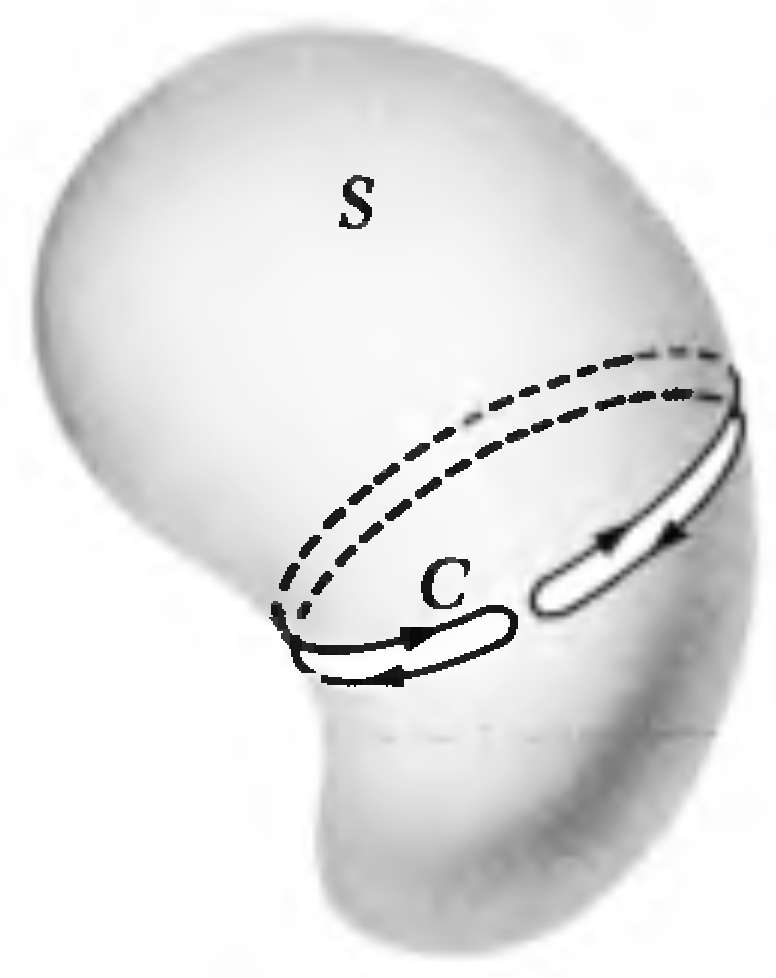
\includegraphics[width=0.33\textwidth]{ps03_02}\end{center}
  \end{enumerate}
\section{Problem \thesection: Stokes's Theorem in Action}
  Consider the vector field $\vec{F} = \hat{x} z^2 + \hat{y} x^2 - \hat{z} y^2$.
  \begin{enumerate}[(a)]
    \item Calculate $\oint \vec{F} \cdot d\vec{r}$ around a square path with
      corners $(x_0 \pm s/2,~~y_0 \pm s/2,~~0)$. The square has
      center $(x_0,y_0,0)$, side length $s$, and its sides are parallel to
      the $x$- and $y$-axes. The sense of rotation of the path
      is counter-clockwise as viewed from the $+z$ direction.
    \item Divide your answer to (a) by the area of the square, and take
      the limit as $s\rightarrow 0$.
    \item Calculate $\vec{\nabla}\times \vec{F}$ at the center of the square.
    \item Verify that your answer to (b) is equal to the normal component
      of $\vec{\nabla}\times\vec{F}$ evaluated at the center of the square.
  \end{enumerate}
\section{Problem \thesection: Gauss's Theorem in Action}
  Consider a vector field
  $\vec{F} = r\hat{r}$ (in spherical coordinates), and a closed
  surface $S$ that is a cube with one corner at the origin and the
  opposite corner at $(b,b,b)$.  Verify Gauss's theorem,
  $$\oint \vec{F}\cdot\hat{n}\,dS = \int (\vec{\nabla}\cdot\vec{F})\,dV,$$
  for this particular case by performing both the surface integral on the
  left side, and the volume integral on the right side, and showing that
  they are equal.
\section{Problem \thesection: Purcell 2.4 \& 2.8}
  \begin{enumerate}[(a)]
    \item Describe the charge distribution that goes with the following potential:
      \begin{align*}
        \phi & = x^2 + y^2 + z^2 & \text{for }x^2 + y^2 + z^2 < a^2 \\
        \phi & = -a^2 + \frac{2a^3}{(x^2 + y^2 + z^2)^{1/2}} & \text{for }a^2 < x^2 + y^2 + z^2
      \end{align*}
      Discuss what happens at the boundary ($x^2 + y^2 + z^2 = a^2$).
    \item Consider a very long cylinder of radius $R$ that is filled with a uniform charge density $\rho$ (Fig. 2.17).  Use the following two different approaches to find the electric field, $\vec{E}$, both inside and outside the cylinder.
      \begin{enumerate}[(i)]
        \item Apply Gauss' law
        \item Integrate Poisson's equation: $\vec{\nabla} \cdot \vec{E} = 4 \pi \rho$.
      \end{enumerate}
      Be sure that the $\vec E$ field inside and the $\vec E$ field outside match at the boundary (i.e., at $R$).
      \begin{center}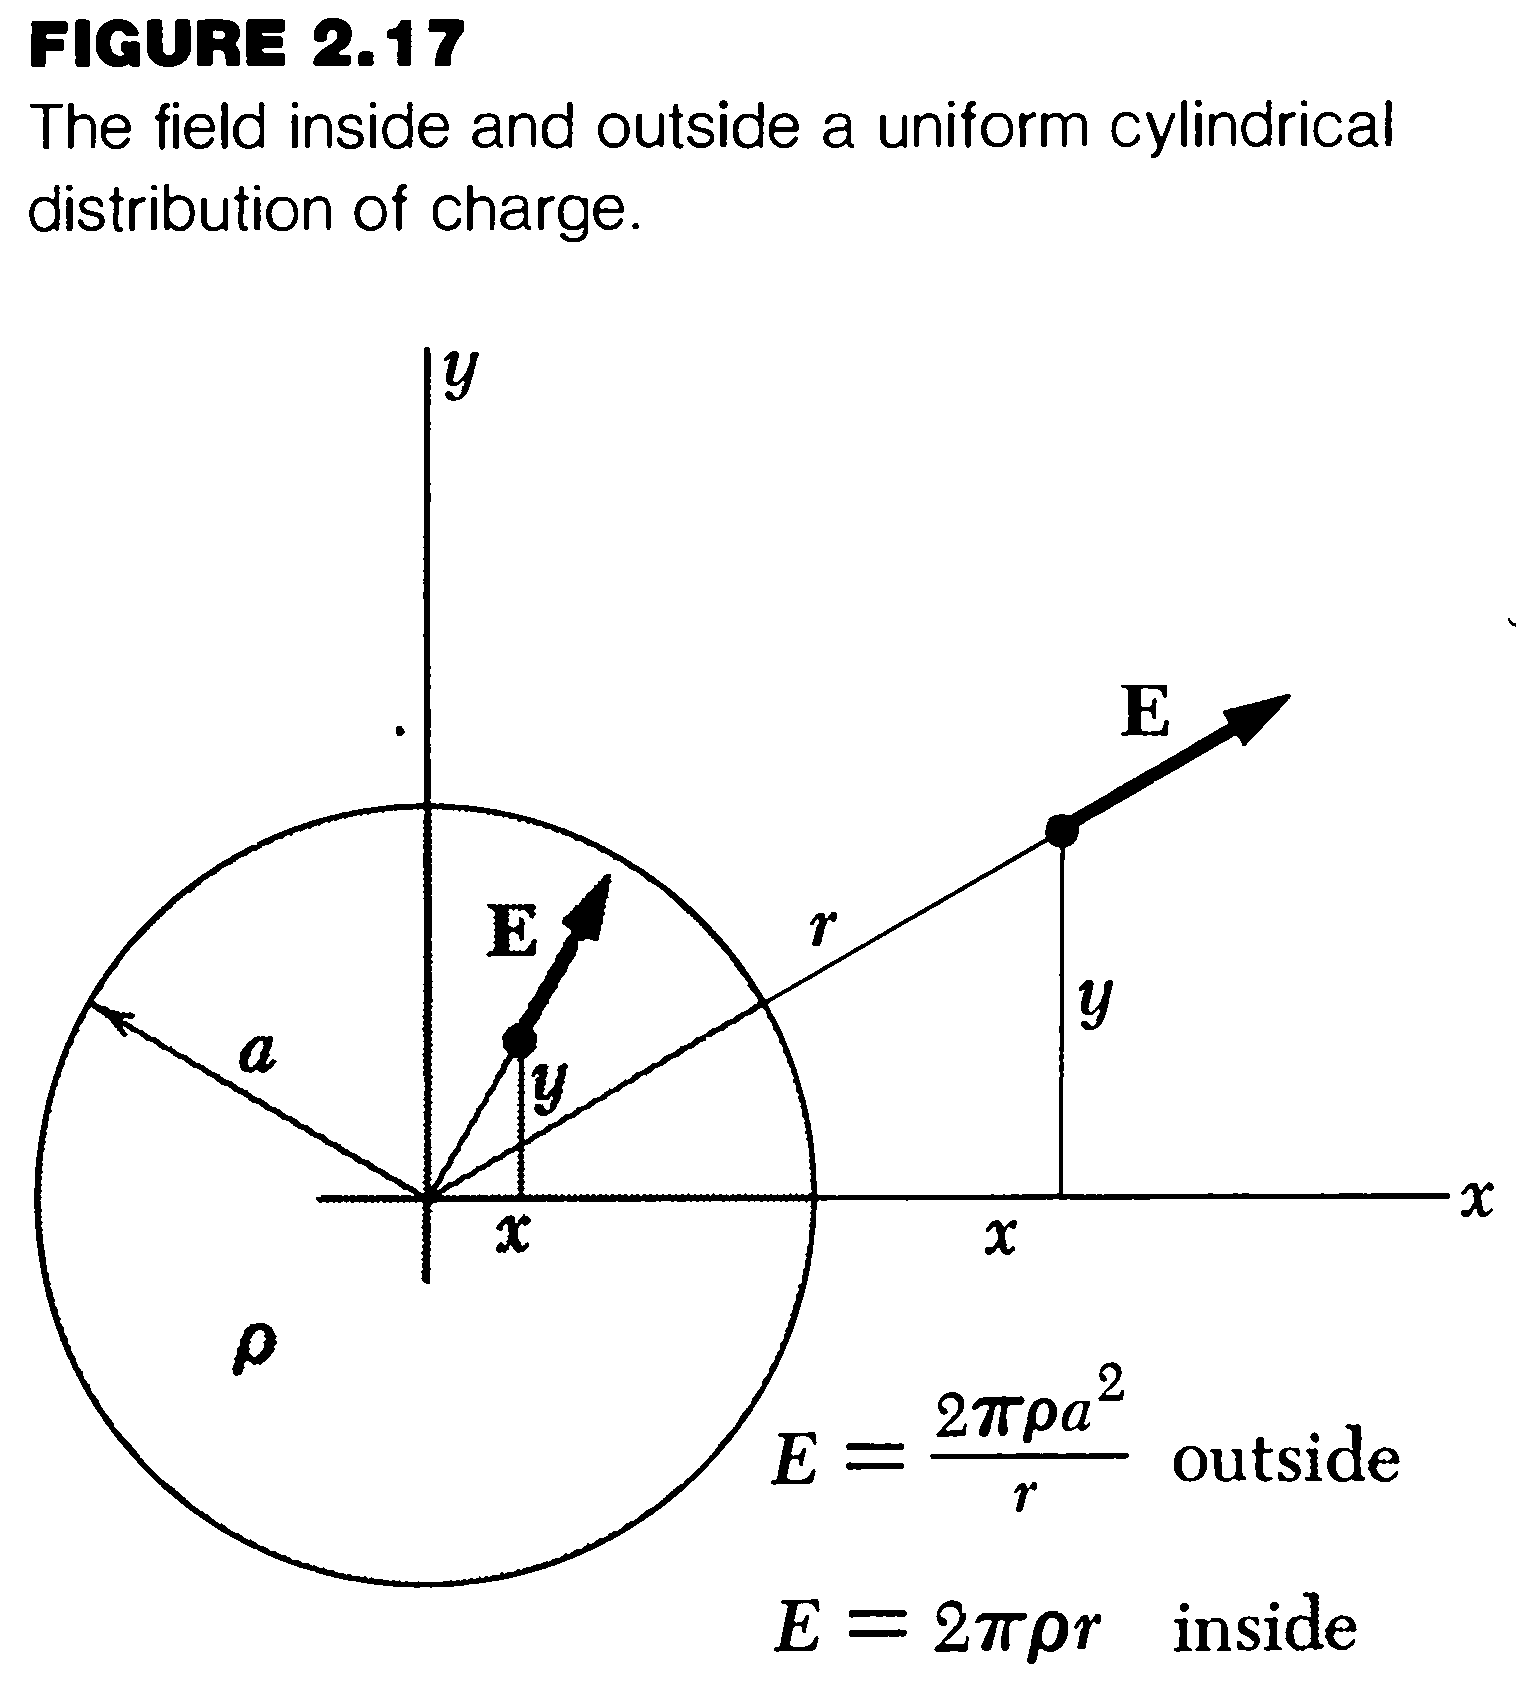
\includegraphics[width=0.5\textwidth]{ps02_2}\end{center}
  \end{enumerate}
\section{Problem \thesection: Potential of an Electric Dipole}
  Compute the potential $\varphi(x,y,z)$ of a dipole charge configuration.  The dipole consists of a charge $+q$ located at $z = a/2$ and a charge $-q$ located at $z=-q$.
  \begin{enumerate}[(a)]
    \item Write down $\varphi(x,y,z)$ (i.e., in Cartesian coordinates).
    \item Expand $\varphi(x,y,z)$ in a Maclaurin series (i.e., a Taylor series about $a=0$) to first order in $a$.
    \item Convert your results to spherical coordinates: $\varphi(r, \theta, \phi)$.
    \item Compute $\vec{\nabla}\varphi(r, \theta, \phi)$, in spherical coordinates, to find $\vec{E}$. % and compare your results with what you found in Problem \#6 of pset \#1.
  \end{enumerate}
\section{Problem \thesection: Purcell 2.29}
  One of two nonconducting spherical shells of radius $a$ carries
  a charge $Q$ uniformly distributed over its surface, the other a charge
  $-Q$, also uniformly distributed. The spheres are brought together
  until they touch. What does the electric field look like, both outside
  and inside the shells? How much work is needed to move them far
  apart?
\section{Problem \thesection: Purcell 2.14 (Laplace's equation)}
  Does the function $f(x, y) = x^2 + y^2$ satisfy the two-dimensional
  Laplace equation? Does the function $g(x, y) = x^2 - y^2$?
  Sketch the latter function, calculate the gradient at the points $(x = 0, y = 1)$;
  $(x = 1, y = 0)$; $(x = 0, y = -1)$; and $(x = -1, y = 0)$ and indicate
  by little arrows how these gradient vectors point.
\section{Problem \thesection: Electric field, potential, and flux}
  A hollow spherical shell carries charge density $\rho = k/r^2$ in the
  region $a \le r \le b$:
  \begin{center}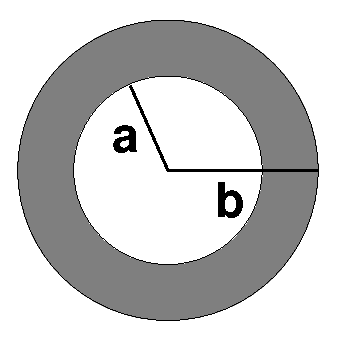
\includegraphics[width=3.5cm]{ps03_09}\end{center}
  \begin{enumerate}[(a)]
    \item Find the electric field $\vec E$ everywhere in space
    \item Find the potential $\phi$ everywhere in space.
    \item Calculate the electric flux through
      \begin{enumerate}[(i)]
        \item A concentric sphere with radius $r_1 > b$
        \item A concentric sphere with radius $a \le r_2 \le b$
        \item A concentric sphere with radius $r_3 < a$
        \item A nonconcentric sphere centered on \emph{any} point on the
          outer surface of the shell, and of radius $r_4 = 2b$.
      \end{enumerate}
  \end{enumerate}
\section{Problem \thesection: Purcell 2.20 (Optional) (Potential at the center of a gold nucleus)}
  As a distribution of electric charge, the gold nucleus can be
  described as a sphere of radius \SI{6e-13}{\centi\meter} with a charge $Q = 79e$
  distributed fairly uniformly through its interior. What is the potential
  $\phi_0$ at the center of the nucleus, expressed in megavolts? (First derive
  a general formula for $\phi_0$ for a sphere of charge $Q$ and radius $a$. Do
  this by using Gauss's law to find the internal and external electric field
  and then integrating to find the potential.)
  \begin{flushright} \emph{Ans}. $\phi_0 = 3Q/2a = \num{95000}\text{ statvolts} = 28.5\text{ megavolts}$. \end{flushright}
\end{document}
